\section{Pre-processing}

The data is extracted from an ascii text file using regular pythonic techniques. This extracted data has a lot of unnecessary data in the beginning of the text file which is easily filtered by identifying the line at which the junk part of the data ends. The rest of the data set (after the 7th for this dataset) is a list of sequences with one line containing one sequence.

The dataset contains nearly one million sequences and the algorithm takes a lot of time to run on the entire dataset. For quick and efficient testing, the dataset is sampled using random sampling.

After sampling, the sequential data needs to be converted to vertical format as required by the SPADE algorithm. The organization of containing one sequence per row is known as horizontal data format - the format in which the dataset is available. To convert this into vertical format, we need to arrange each unique event present in the dataset as shown in Fig. \ref{vertical}. Each event is represented as a list of tuples, each tuple contains the sequence ID and event ID of the event occurrence and all the tuples together represent all the occurrences of the event.

\begin{figure}[h]
    \centerline{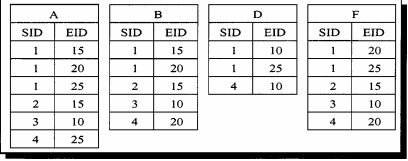
\includegraphics[width=0.5\textwidth]{figures/vertical_data.png}}
    \caption{Example of a vertical dataset}
    \label{vertical}
\end{figure}